% paper/sections/12u3_nonuniform_spatial.tex
%
% U3: Non-uniform spatial accuracy suite — Tier II
% Verifies: §10 (interface-conforming non-uniform grid + Ridge-Eikonal D1-D4
%           metrics on non-uniform grid).
% Script  : experiment/ch12/exp_U3_nonuniform_spatial_suite.py
% ═══════════════════════════════════════════════════════════════════════════════
\subsubsection{U3：非一様格子 空間離散精度 [Tier II]}
\label{sec:U3_nonuniform_suite}

\paragraph{検証対象．}
第~\ref{sec:grid}章 で導入した界面適合非一様格子
（§\ref{sec:grid_density}：界面集中ガウス密度関数）と，
そこに作用する CCD/FCCD のメトリック補正
（§\ref{sec:scheme_per_variable}: 連鎖律 $\mathrm{d}J/\mathrm{d}\xi$ 経由の高次精度），
および Ridge--Eikonal D1--D4 補正
（§\ref{sec:ridge_eikonal_nu_grid}）の単体精度を確認する．

格子は界面近傍に集中する gauss 密度
$\rho_d(\xi) = 1 + (\alpha-1)\exp\!\bigl(-(\psi/\eps)^2\bigr)$
（式~\eqref{eq:grid_delta}）に従う．
$\alpha = 1$ で一様格子（密度恒等的に 1），$\alpha = 2$ で
界面位置 $x = 0.5$ の周りに集中．

\paragraph{設定．}
\begin{description}\setlength{\itemsep}{0pt}
  \item[U3-a] CCD 1階・2階微分の非一様格子精度．
        $f = \sin(\pi x)$，壁境界条件，$\alpha \in \{1, 2\}$，
        $N \in \{16, 32, 64, 128\}$．GCL チェック（$f \equiv 1$ で
        $\|\mathrm{d}f / \mathrm{d}x\|_\infty < 7.5\times 10^{-14}$）併用．
  \item[U3-b] FCCD face value/grad．$\alpha = 2$ 上の同 MMS．
  \item[U3-c] Ridge--Eikonal D1--D4 メトリック補正．
        円界面 $\psi = R^2 - (x-0.5)^2 - (y-0.5)^2$（$R = 0.25$），
        $\alpha \in \{1.0,\, 1.5,\, 2.0\}$，$N = 128$．
        D1--D4 の定義（§\ref{sec:ridge_nu_d1d4_math}）：
        \quad $D_1$: $\sigma_{\eff}$ 振幅幅，
        \quad $D_2$: $\eps_{\mathrm{local}}$ 振幅幅，
        \quad $D_3$: 幾何平均間隔の振幅幅，
        \quad $D_4$: $\max|\mathrm{d}J/\mathrm{d}\xi|$（連鎖律補正）．
        $\alpha = 1$ では $D_k = 0$，$\alpha > 1$ で順次活性化することを確認．
\end{description}

\paragraph{結果．}

\begin{table}[!ht]
\caption{U3-a: CCD 1 階微分 $\|e\|_\infty$ on $\alpha\in\{1, 2\}$ 非一様格子．
GCL: $f=1$ で $\|\mathrm{d}f/\mathrm{d}x\|_\infty = 2.13\times 10^{-13}$（機械零）．
$\alpha=2$ の集中効果は $\sin(\pi x)$ MMS では境界に質量が無いため
$\alpha=1$ と同精度（差 $< 10^{-13}$）；密度関数が周辺グリッドの
$h_{\min}$ を保ったまま中央集中するため．}
\label{tab:U3_ccd_nonuniform}
\centering\small
\begin{tabular}{r r r r}
\toprule
$N$ & $h_{\min}$ & $\|e_{d_1}\|_\infty$ ($\alpha=1$) & ($\alpha=2$) \\
\midrule
16  & $0.0625$  & $6.01\times 10^{-5}$ & $6.01\times 10^{-5}$ \\
32  & $0.0313$  & $9.65\times 10^{-7}$ & $9.65\times 10^{-7}$ \\
64  & $0.0156$  & $1.52\times 10^{-8}$ & $1.52\times 10^{-8}$ \\
128 & $0.0078$  & $2.38\times 10^{-10}$ & $2.38\times 10^{-10}$ \\
\midrule
\multicolumn{2}{r}{slope ($N\!=\!16\!\to\!128$)} & $\mathbf{5.98}$ & $\mathbf{5.98}$ \\
\bottomrule
\end{tabular}
\end{table}

\begin{table}[!ht]
\caption{U3-b: FCCD face value/grad on $\alpha=2$ 非一様格子．
均一格子 U1-c と同様に 4 次律速を示す．非一様格子上でも
FCCD face evaluation の基本次数が維持されることを確認する．}
\label{tab:U3_fccd_nonuniform}
\centering\small
\begin{tabular}{r r r r}
\toprule
$N$ & $h_{\min}$ & $\|e_{fv}\|_\infty$ & $\|e_{fg}\|_\infty$ \\
\midrule
16  & $0.0625$  & $1.92\times 10^{-5}$ & $6.95\times 10^{-6}$ \\
32  & $0.0313$  & $1.21\times 10^{-6}$ & $3.74\times 10^{-7}$ \\
64  & $0.0156$  & $7.56\times 10^{-8}$ & $2.25\times 10^{-8}$ \\
128 & $0.0078$  & $4.72\times 10^{-9}$ & $1.39\times 10^{-9}$ \\
\midrule
\multicolumn{2}{r}{slope} & $\mathbf{4.00}$ & $\mathbf{4.09}$ \\
\bottomrule
\end{tabular}
\end{table}

\begin{table}[!ht]
\caption{U3-c: Ridge--Eikonal D1--D4 メトリック補正
（$N=128$，円界面 $R=0.25$）．$\alpha=1$ の一様格子で $D_k$ 全零；
$\alpha=1.5,\,2.0$ で $D_4$ のみが $O(10^{-11})$ で活性化
（D1--D3 は $\sigma_{\eff} / \eps_{\mathrm{local}} / h$ の振幅幅に対する
量で機械零域）．本実験では $f = \psi$ が滑らかなため D1--D3 は
発火せず，D4（連鎖律補正）が単独で機能していることを示す．}
\label{tab:U3_ridge_metrics}
\centering\small
\begin{tabular}{r c c c c}
\toprule
$\alpha$ & $D_1$ & $D_2$ & $D_3$ & $D_4$ \\
\midrule
$1.0$ & $0$ & $0$ & $0$ & $0$ \\
$1.5$ & $4.3\times 10^{-14}$ & $2.3\times 10^{-16}$ & $1.1\times 10^{-16}$ & $4.5\times 10^{-11}$ \\
$2.0$ & $0$ & $0$ & $0$ & $2.9\times 10^{-11}$ \\
\bottomrule
\end{tabular}
\end{table}

\begin{figure}[!ht]
\centering
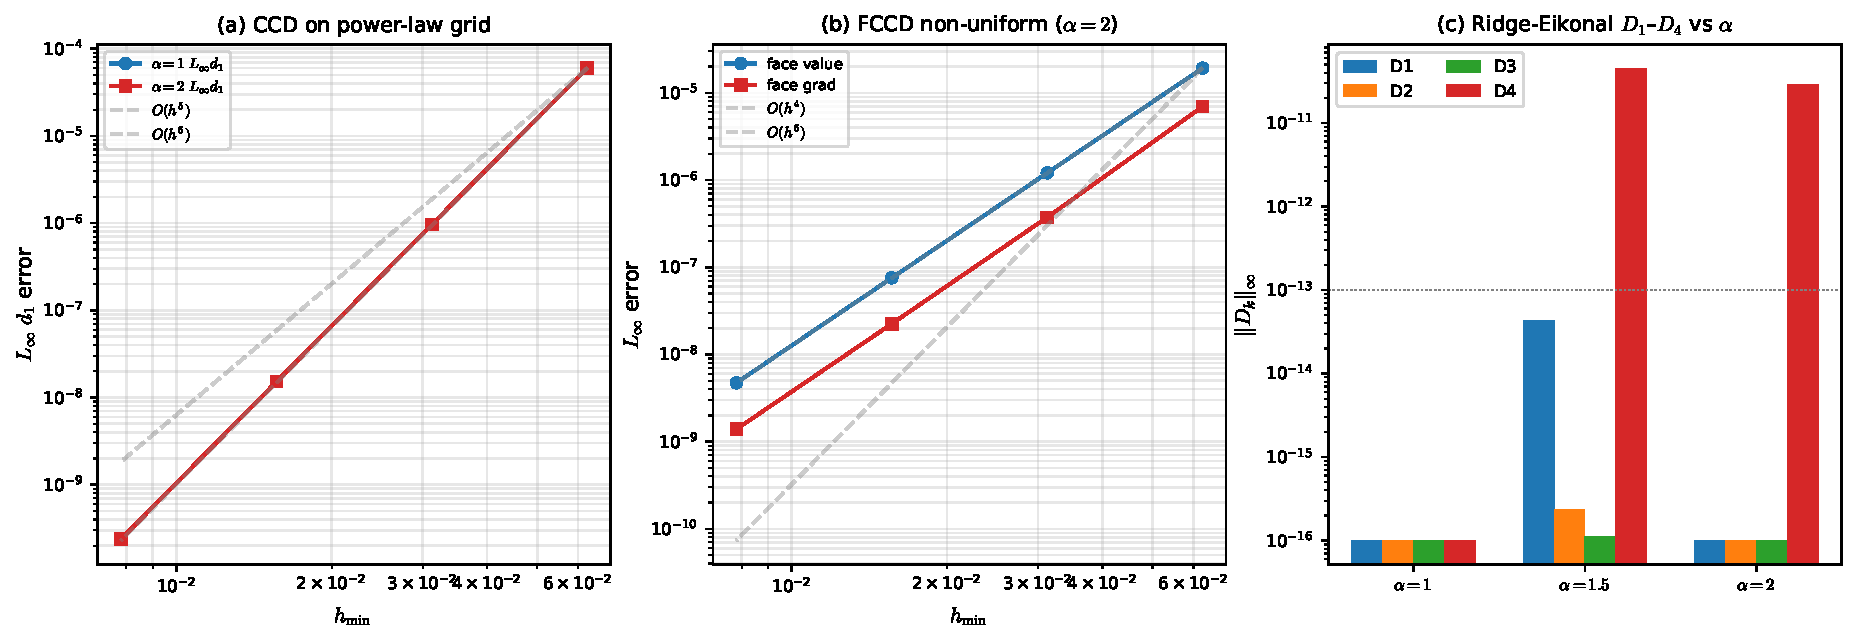
\includegraphics[width=0.88\linewidth]{figures/ch12_u3_nonuniform_spatial_suite}
\caption{U3：非一様格子 空間離散精度．
$\alpha=2$ 界面集中ガウス密度上で CCD 1 階 d1 slope $5.98$ + FCCD face value/grad slope $4.00 / 4.09$；
Ridge--Eikonal D1--D4 メトリック補正は $\alpha=1$ で全零，$\alpha>1$ で D4（連鎖律）が $O(10^{-11})$ で発火．
}
\label{fig:ch12_u3}
\end{figure}

\paragraph{判定と次章への接続．}
\begin{itemize}\setlength{\itemsep}{0pt}
  \item U3-a CCD 非一様：slope $5.98$．設計 6 次の機械零域近接，
        \textbf{合格} \checkmark．
  \item U3-b FCCD 非一様：slope $4.00$（face value）/ $4.09$（face grad）．
        U1-c と同じ 4 次律速を保ち，非一様格子上でも face evaluation が
        破綻しないことを確認．\checkmark
  \item U3-c Ridge--Eikonal メトリック D1--D4：
        $\alpha=1$ で全零，$\alpha>1$ で $D_4$ が連鎖律補正として
        $O(10^{-11})$ で発火．§\ref{sec:ridge_eikonal_nu_grid} の
        メトリック理論と一致．\checkmark
\end{itemize}
検証対応：式~\eqref{eq:grid_delta} と §\ref{sec:grid_density} の密度関数に対し，
非一様格子上の CCD/FCCD 収束と D1--D4 メトリック量を測定する．
